\section*{Описание схемы распараллеливания}
\addcontentsline{toc}{section}{Описание схемы распараллеливания}

На вход подается одномерный массив пикселей размера $m\cdot n$. Благодаря этому массив хранится линейно в оперативной памяти, что дает нам большое преимущество в распределении определенных блоков между процессами при помощи функции \textbf{MPI\textunderscore Scatterv} (рис.\ref{fig:distrImage}).

\vspace{5mm}

\begin{figure}[h!]
\centering
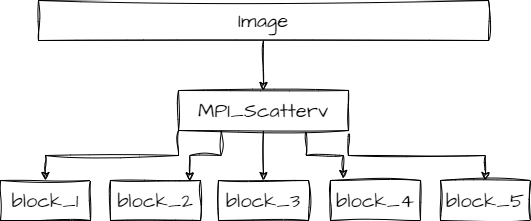
\includegraphics[width=0.8\textwidth]{images/distrImage.png}
\caption{Распределение изображения между 5 процессами.}
\label{fig:distrImage}
\end{figure}

\vspace{5mm}

После того, когда на каждом процессе будет свой участок изображения, нам необходимо найти максимальное и минимальное значение пикселей. Затем при помощи функции \textbf{MPI\textunderscore Allreduce} редуцировать все локальные результаты по операциям \textbf{MPI\textunderscore MAX} и \textbf{MPI\textunderscore MIN} соответсвенно (рис. \ref{fig:allreduce}).

\vspace{5mm}

\begin{figure}[h!]
\centering
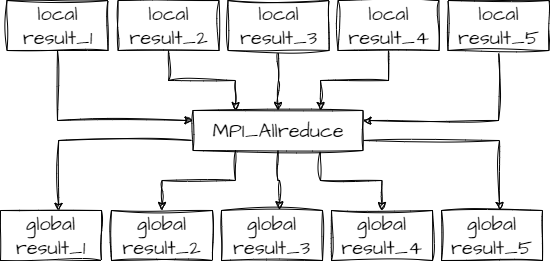
\includegraphics[width=0.8\textwidth]{images/MPI_Allreduce.png}
\caption{Редуцирование 5 процессов.}
\label{fig:allreduce}
\end{figure}

\vspace{5mm}

Следующим этапом будет вызов последовательной версии алгоритма для каждого из процессов, где каждый пиксель будет обработан по формуле, которая была указана ранее (\ref{formulaLinStreach}).

\vspace{2cm}

Самым последним действием будет сбор и объединение полученных локальных изображений при помощи функции \textbf{MPI\textunderscore Gatherv} (рис.\ref{fig:gatherv}).

\vspace{5mm}

\begin{figure}[h!]
\centering
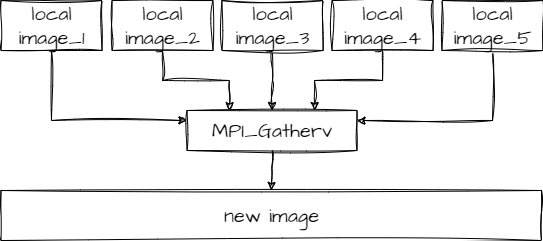
\includegraphics[width=0.8\textwidth]{images/gatherv.png}
\caption{Объединение 5 локальных изображений в результирующее.}
\label{fig:gatherv}
\end{figure}
